\documentclass[letter]{scrartcl}
\usepackage{graphicx}
\usepackage{fullpage} %1in margins
\usepackage{tabularx}
\usepackage{hyperref}
\usepackage{tikz} % for diagrams
\usetikzlibrary{automata,positioning}

\newcommand{\app}{\sc{393torrent}}

\begin{document}

\title{Requirements for \app}
\subtitle{Dan Keller, Kenneth Link, Nathan McKinley, Ross Nanopoulos}
\date{} % no date

\maketitle

\begin{abstract}
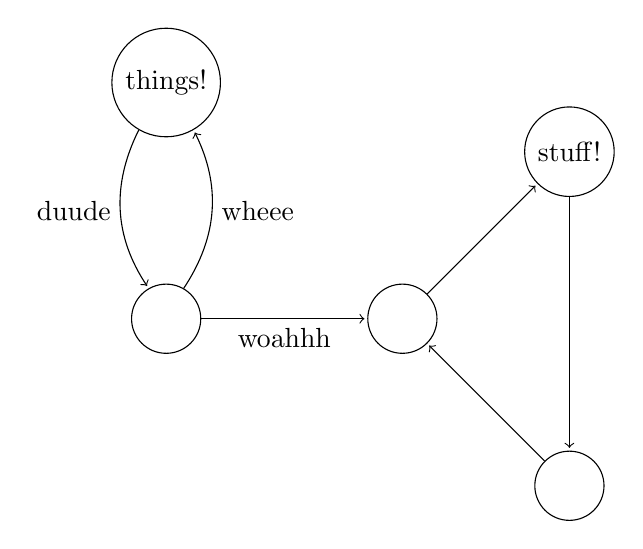
\begin{tikzpicture}[shorten >=1pt,node distance=3cm,on grid,auto]
	\node[state] (s) {};
	\node[state] (a1) [above=of s] {things!};
	\node[state] (b1) [right=of s] {};
	\node[state] (b2) [above right=of b1] {stuff!};
	\node[state] (b3) [below right=of b1] {};
	\path[->]
	(s)  edge [bend right] node [right] {wheee} (a1)
	     edge node [below] {woahhh} (b1)
	(a1) edge [bend right] node [left] {duude} (s)
	(b1) edge node {} (b2)
	(b2) edge node {} (b3)
	(b3) edge node {} (b1);
\end{tikzpicture}

The software requirements specification (SRS) specifies all user stories (i.e. functional requirements) as well as nonfunctional requirements. These requirements are used in iteration planning as well as acceptance testing.  This document should be used by the members of the 393torrent team, who will implement and verify the functionality of the BitTorrent client.
\end{abstract}

\tableofcontents
\pagebreak

\section{Overview}
The BitTorrent client (393torrent) will allow users to download, create, and seed torrent files.  It will enable them to achieve the full functionality of a BitTorrent client in a lightweight form.  The primary objective of this BitTorrent client is to offer a free and open source alternative--without advertisements--to the current heavyweight clients available.  Specific goals of 393torrent can be found in the vision and scope document.

\section{Protocol}
Bittorrent Protocol

\subsection{Protocol Overview}
	
Bittorrent is a file transfer protocol created by Bram Cohen intended for sending files over unreliable networks.  A torrent is a collection of peers who are participating in the distribution of a file.  To achieve a reliable download protocol over unreliable networks, bittorrent uses many peers who send and receive small equi-sized “chunks” of data (typically 256KB).  A peer joins a torrent by registering with something called the tracker.  The tracker keeps track of all peers participating in the torrent and requires updates from each peer to continue tracking them.  The number of peers can be anything from one to thousands of peers, however the more peers the faster the download speed which is opposite of server hosted downloads.  After the tracker becomes aware of a new peer it sends that user (User A) a list of ip addresses of other peers on the torrent.  User A will attempt to connect via TCP to each of the peers obtained from the list and exchange a list of missing chunks with that peer.  With the new knowledge of which peer has the chunks that User A is missing, User A can request the rarest chunks first (a chunk that most of her peers do not have but at least one peer does have).  After the rarest first have been taken care of, User A will continue trading chunks with peers who are currently supplying User A with the highest data rate.  Also, every 10 seconds User A will recalculate the download rates and update the list of highest data rate peers.  Additionally every 30 seconds User A chooses one peer by random and sends a chunk to it. 

\subsection{Tracker}
	The tracker is a database of peers which responds to HTTP GET requests.  These requests can return tracker statistics and a list of peer ip addresses. Typical tracker requests may include the following parameters:
info\_hash: urlencoded 20-byte SHA1 hash of the value of the info key from the Metainfo file
peer\_id: urlencoded 20-byte string used as a unique ID for the client, generated by the client at startup
port: The port number that the client is listening on
uploaded: The total amount uploaded (since the client sent the 'started' event to the tracker) in base ten ASCII.
downloaded:  The total amount downloaded (since the client sent the 'started' event to the tracker) in base ten ASCII
left: The number of bytes this client still has to download in base ten ASCII.
compact: Setting this to 1 indicates that the client accepts a compact response.
no\_peer\_id: Indicates that the tracker can omit peer id field in peers dictionary
event:  If specified, must be one of started, completed, stopped, (or empty which is the same as not being specified). If not specified, then this request is one performed at regular intervals.
ip: Optional. The true IP address of the client machine, in dotted quad format or rfc3513 defined hexed IPv6 address
numwant: Optional. Number of peers that the client would like to receive from the tracker. This value is permitted to be zero. If omitted, typically defaults to 50 peers.
key: Optional. An additional client identification mechanism that is not shared with any peers. It is intended to allow a client to prove their identity should their IP address change.
trackerid: Optional. If a previous announce contained a tracker id, it should be set here.

Trackers answer a request with a response containing a plaintext document which contains a bencoded dictionary with these keys:
failure reason: If present, then no other keys may be present. The value is a human-readable error message as to why the request failed (string).
warning message: (new, optional) Similar to failure reason, but the response still gets processed normally. The warning message is shown just like an error.
interval: Interval in seconds that the client should wait between sending regular requests to the tracker
min interval: (optional) Minimum announce interval. If present clients must not reannounce more frequently than this.
tracker id: A string that the client should send back on its next announcements. If absent and a previous announce sent a tracker id, do not discard the old value; keep using it.
complete: number of peers with the entire file, i.e. seeders (integer)
incomplete: number of non-seeder peers, aka "leechers" (integer)
peers: (dictionary model) The value is a list of dictionaries, each with the following keys:
peer id: peer's self-selected ID, as described above for the tracker request (string)
ip: peer's IP address either IPv6 (hexed) or IPv4 (dotted quad) or DNS name (string)
port: peer's port number (integer)
peers: (binary model) Instead of using the dictionary model described above, the peers value may be a string consisting of multiples of 6 bytes. First 4 bytes are the IP address and last 2 bytes are the port number. All in network (big endian) notation.

\subsection{Peer Wire Protocol TCP}

In TCP, a client must remember state information such as:

choked: When a peer uses the choke signal, it is letting the other peer’s client know that notification requests will not be answered unless the client is unchoked. 
interested: If the client is interested in the 

X. Advantages

As opposed to traditional file distribution methods, Bittorrent has fasted distribution time which increases as the number of users increases because a high number of peers means there  will be a more efficient use of bandwidth. 

Wiki.theory.org Contributors. (2013 July 26) “Bittorrent Protocol Specification v1.0”. [Online]. Available: https://wiki.theory.org/BitTorrentSpecification

Ross Kurose. “Chapter 2 Application Layer”. Computer Networking A Top-Down Approach 6th edition

\section{App Architecture}

\section{Thread Model}

\section{Classes in Detail}

\pagebreak
\section{Author Contributions}
This section provides the details to what each author contributed to the vision and scope document, as requested per professor Podgurski.
\subsection{Daniel Keller}
Created document outline and 
\subsection{Kenneth Link}

\subsection{Nathan McKinley}

\subsection{Ross Nanopoulos}


\section{Inspection}
\begin{tabularx}{\textwidth}{X c c}
\textbf{Comment} & \textbf{Reported By} & \textbf{Fixed By} \\
\end{tabularx}
\end{document}
